\documentclass{article}
\usepackage[utf8]{inputenc}
\usepackage{amssymb,amsmath}
\usepackage[parfill]{parskip}
\DeclareMathOperator*{\argmin}{arg\,min}
\DeclareMathOperator*{\argmax}{arg\,max}
\usepackage{graphicx}
\usepackage{subcaption}

\usepackage{mathtools}
\DeclareMathOperator{\tr}{tr}

\title{Optimization 10/36-725\\
        Homework 2}
\author{Willie Neiswanger}
\date{}

\begin{document}

\maketitle


\section*{Problem Five}


\textbf{(Q1)}

(a) We perform preprocessing with the function normalize\_faces.m.

(b) We plot the columns (faces) of $W$ in Figure 1. We plot the objective value
in every iteration in Figure 2. We can inspect the rows of $H$ to determine
which columns of $W$ were most highly weighted, and thus determine that the
columns of $W$ that encoded face shape seem most important.

\begin{figure}[h!tbp]
        \center{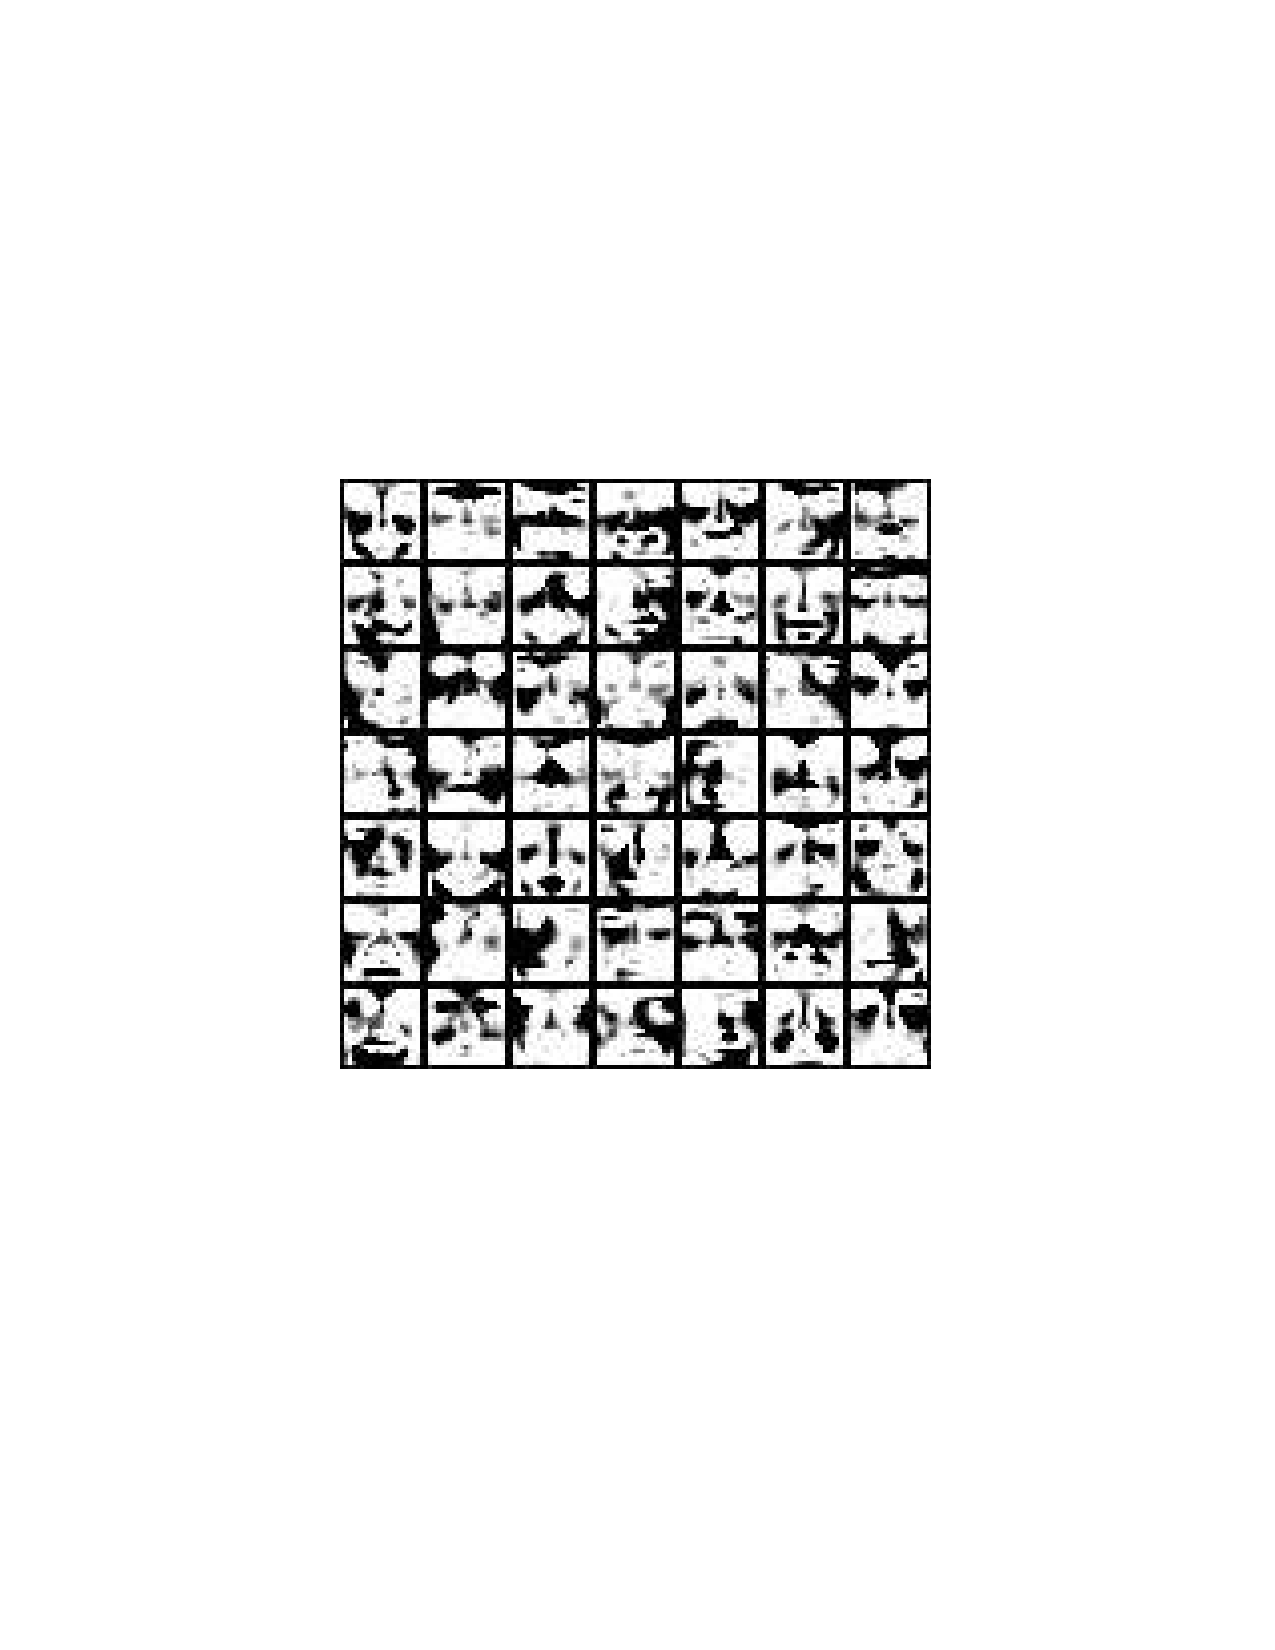
\includegraphics[width=0.7\textwidth]{img/Wmat.pdf}}
        \caption{Faces from the $W$ matrix.}
\end{figure}

\begin{figure}[h!tbp]
        \center{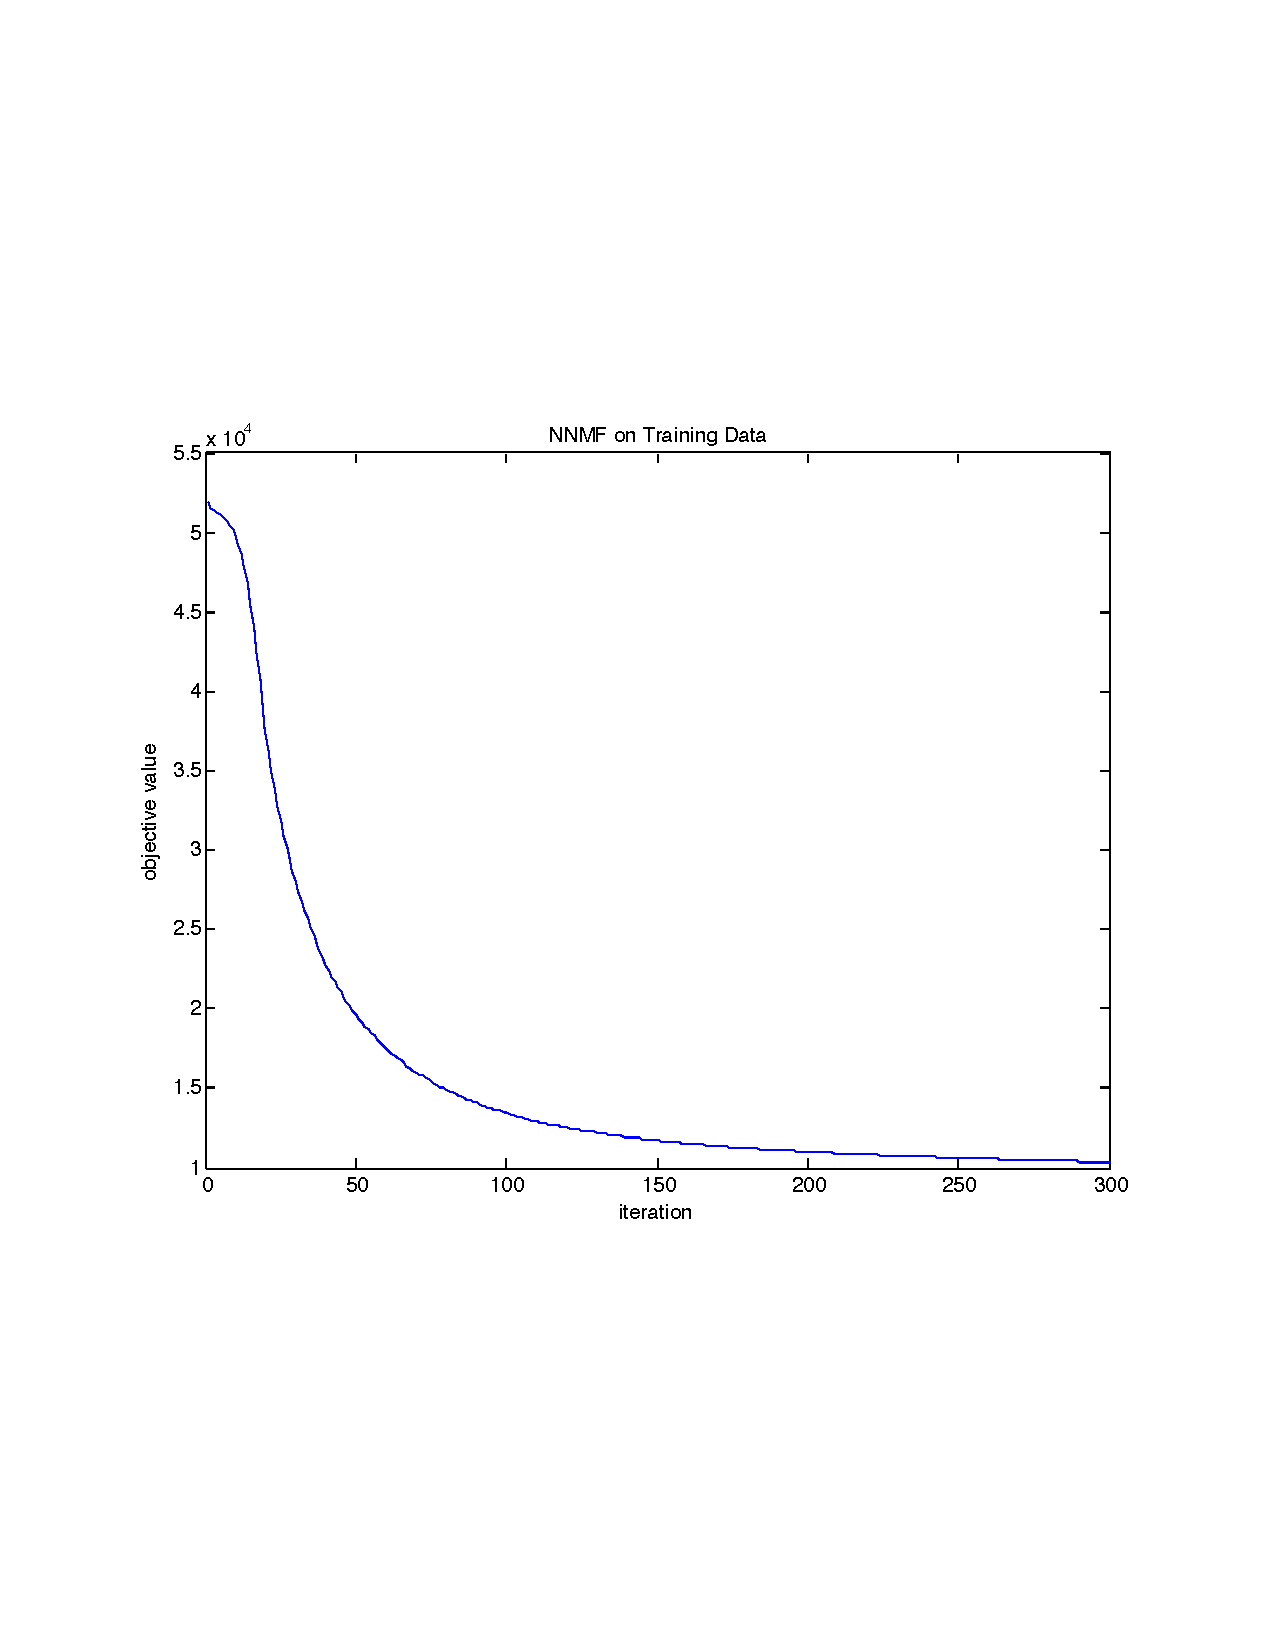
\includegraphics[width=0.7\textwidth]{img/nnmfCurve.pdf}}
        \caption{NNMF error objective values during optimization (on the
        training faces).}
\end{figure}

(c) We can see that this algorithm performs gradient descent updates, where the
authors chooses a step size $t$ such that the additive element in the usual
gradient descent update goes away, and an update for a given matrix turns into
the multiplicative update we see in equation (4). Further, since we initialized
all matrices ($W$ and $H$) to nonnegative values, since $V$ is also
nonnegative, and since all updates consist of multiplication of matrix
elements, we preserve the positive elements during the updates of each matrix.
Hence, we are performing a version of gradient updates where we preserve the
positive elements in each matrix.

An alternative, still using gradient descent, to ensure that the entries of
$W$, $H$ are nonnegative is to take gradient steps and project this back onto
the set of positive matrices at each step (i.e. to carry out projected gradient
descent).

(d) The mean mean-squared-error of the reconstructed images is 6.376.  After
inspection, we see that the reconstructed faces look similar to the test faces
(a few of the faces are even less blurry, and the facial features are more
clear). We show the test and reconstructed faces in Figures 3 and 4.

\begin{figure}[h!tbp]
        \center{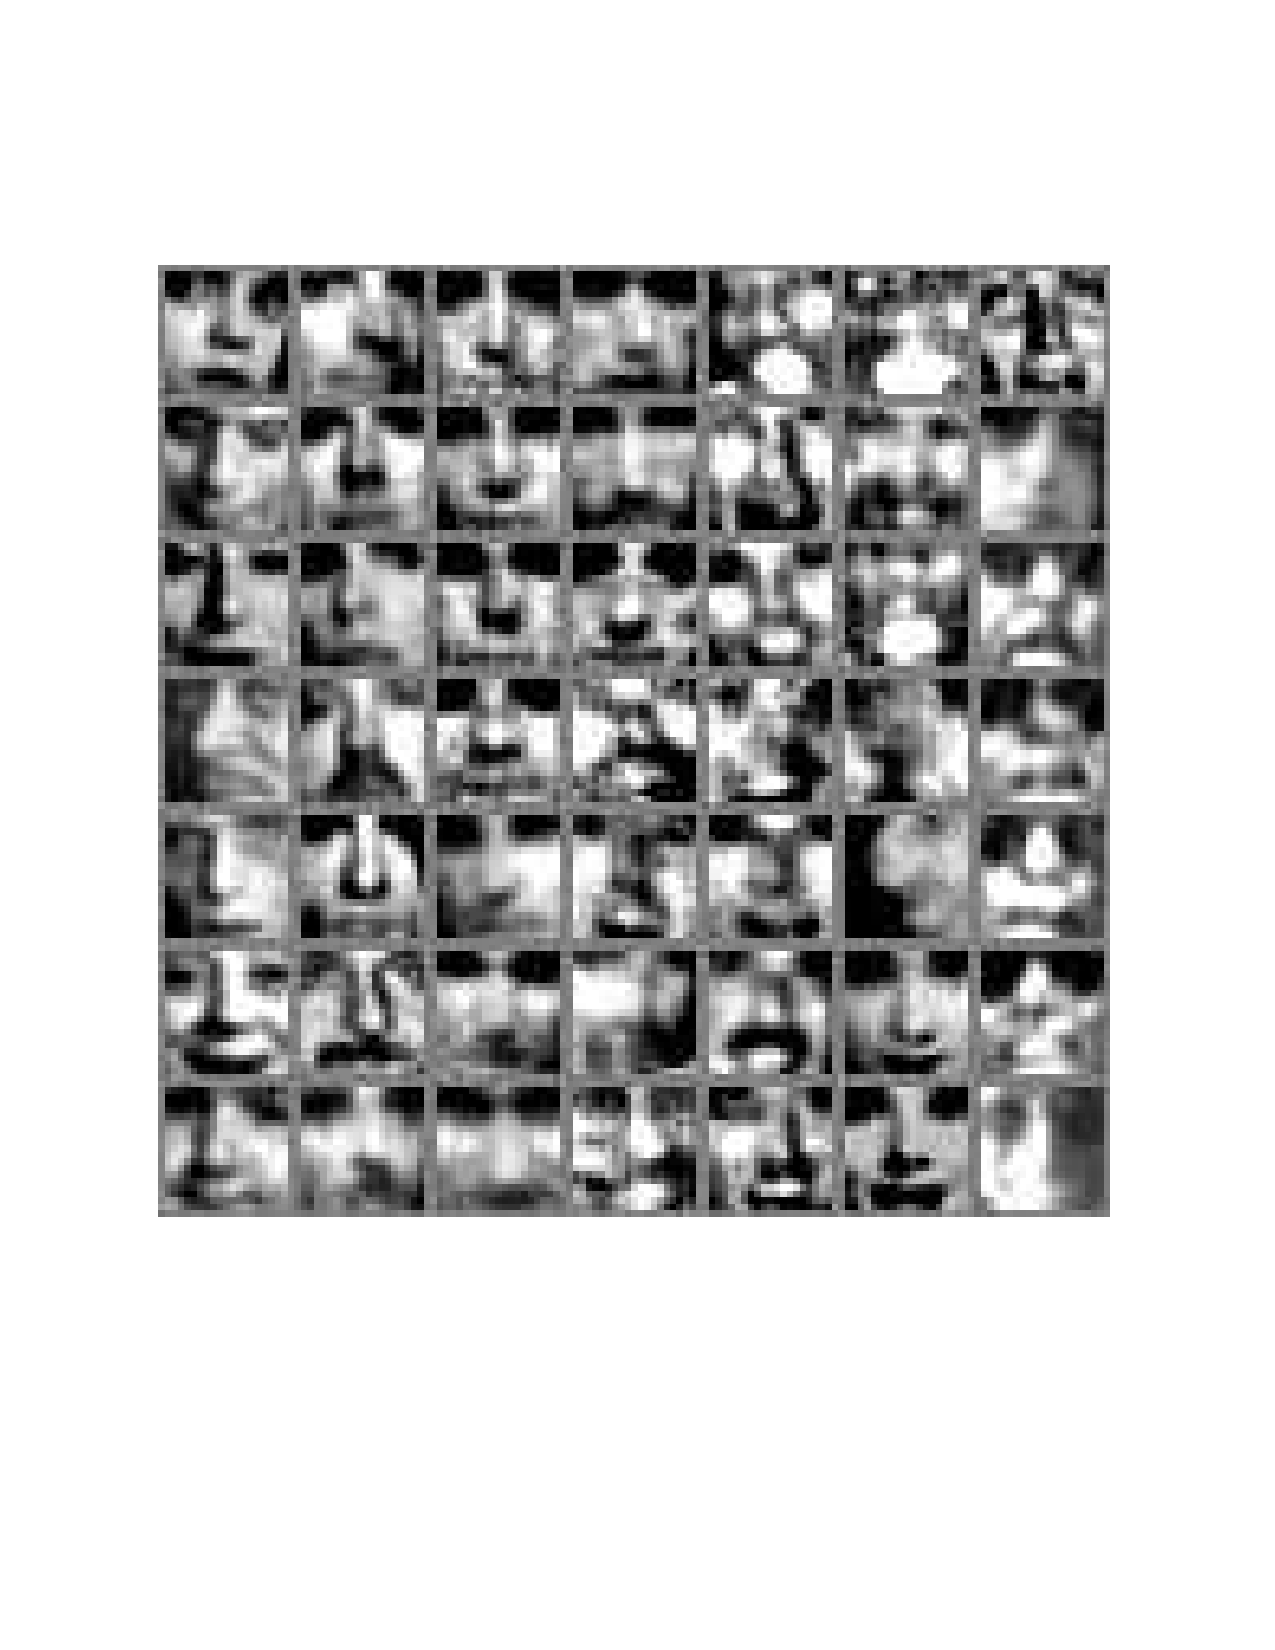
\includegraphics[width=0.7\textwidth]{img/testfaces1.pdf}}
        \caption{Initial test faces.}
\end{figure}

\begin{figure}[h!tbp]
        \center{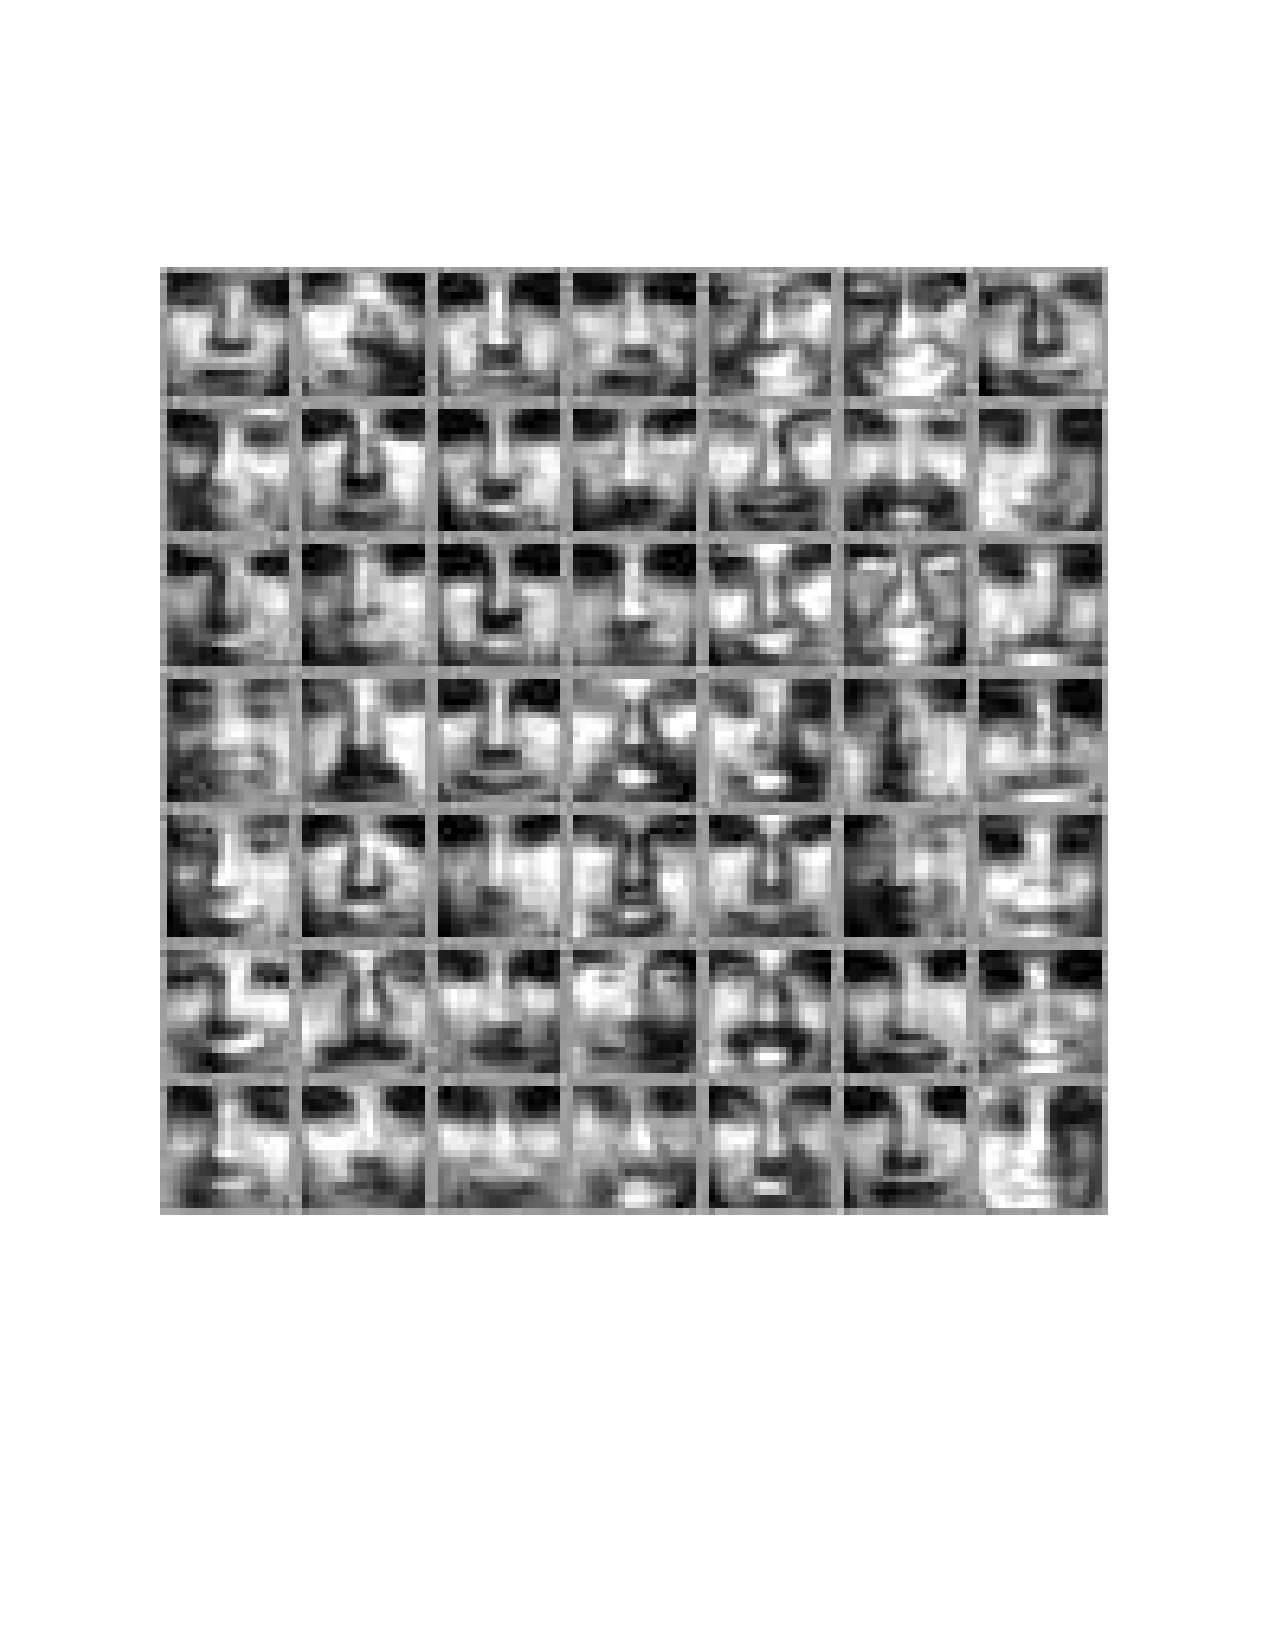
\includegraphics[width=0.7\textwidth]{img/testfaces2.pdf}}
        \caption{Reconstructed test faces.}
\end{figure}

\end{document}
